\section{Methodology}


Explain what methods you used to arrive at your results. For example,
in this work we adopted XKCD's machine learning algorithm. The algorithm is
popularly known as ``linear algebra'' and ``statistics.''
\begin{figure}[h]
	\centering
	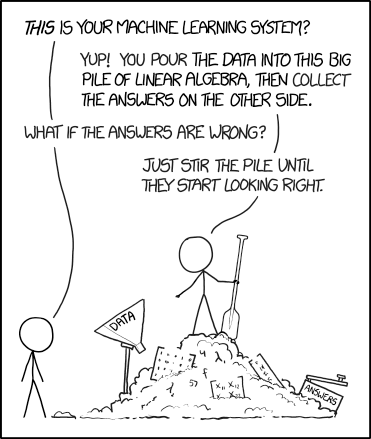
\includegraphics[width=0.65\columnwidth]{machine_learning}
	\caption{Graphical representation of XKCD's algorithm.}
	\label{fig:ML}
\end{figure}

\subsection{This is a subsection}

If you used an equation with ten variables that you need to explain, do it here.

Guidance for equations:
\begin{itemize}
	\item All variables should be one letter.
	\item Use the \texttt{align} environment.
	\item Use \texttt{intertext\{\}} to add text inbetween lines.
	\item Variables should not get their own equation numbers.
	\item Do your best to make the equation a part of a sentence.
\end{itemize}

\begin{align}
 	P_{pv} &= G_T\tau_{pv}\eta_{ref}A[1-\gamma(T-25)]\\
\intertext{where}
	G_T &= I_{DNI}*\cos(\beta+\delta-lat)+I_{DHI}*\frac{180-\beta}{180}\\
	\delta &= 23.44*\sin\left(\frac{\pi}{180}\frac{360}{365}(N+284)\right)
	\intertext{where }
	N &=\mbox{ day of the year}\nonumber\\
	I_{DNI} &=\mbox{ Direct Normal Irradiance [kW]}\nonumber\\
	I_{DHI} &=\mbox{ Diffuse Horizontal Irradiance [kW]}\nonumber\\
	G_T &=\mbox{ total irradiance [kW]}\nonumber\\
	\eta &=\mbox{ conversion efficiency (0.15)}\nonumber\\
	\beta &=\mbox{ tilt of the solar panels [$degrees$]}\nonumber\\
	\delta &=\mbox{ declination of the Earth [$degrees$]}\nonumber\\
	T &=\mbox{ temperature [$^\circ$C]}\nonumber\\
	A &=\mbox{ area covered by solar farm [$m^2$]} \nonumber\\
	\gamma &=\mbox{ temperature coefficient (0.0045)}\nonumber\\
	\tau &=\mbox{ transmittance of the PV module}\nonumber
\end{align}

That's one ugly equation \cite{baker_optimal_2018}.
